\documentclass[review,authoryear,11pt]{elsarticle}

\usepackage[T1]{fontenc}
% sin una familia Type 1 detras, T1 cae en fuentes de mapa de bits (Type 3),
% que las imprentas de Elsevier rechazan
\usepackage{lmodern}
\usepackage{amsmath,amssymb}
\usepackage{booktabs}
\usepackage{graphicx}
\usepackage{xcolor}
\usepackage{multirow}
\usepackage{tikz}
\usepackage{algorithm}
\usepackage{algpseudocode}
\usepackage[expansion=false]{microtype}
% las referencias al material suplementario (S-...) se resuelven con su
% supplementary.aux: compilar supplementary.tex antes que este
\usepackage{xr-hyper}
\usepackage{hyperref}
\externaldocument[S-]{supplementary}

\newcommand{\todo}[1]{\textcolor{red}{[TODO: #1]}}
\newcommand{\RE}{\mathrm{RE}}
\newcommand{\LB}{\mathrm{LB}}

% margen extra para que TeX resuelva parrafos dificiles sin desbordar
\setlength{\emergencystretch}{3em}

% el modo review es a doble espacio, asi que caben pocas lineas por pagina y
% los valores por defecto empujan los floats varias paginas por detras de su
% cita. Se relajan para que una tabla y una figura puedan compartir el top.
\setcounter{topnumber}{3}
\setcounter{totalnumber}{4}
\renewcommand{\topfraction}{.85}
\renewcommand{\textfraction}{.1}
\renewcommand{\floatpagefraction}{.75}

\journal{Computers \& Industrial Engineering}

\begin{document}

\begin{frontmatter}

\title{Genetic Programming Hyper-Heuristics for the Job Shop Scheduling
Problem with Interval Durations: Robustness-Aware Interpretable Rules
that Generalize Across Instance Sizes}

\author{Hern\'an D\'iaz Rodr\'iguez}
\ead{diazhernan@uniovi.es}
\affiliation{organization={Department of Computing, University of Oviedo},
            addressline={Campus de Gij\'on},
            city={Gij\'on},
            postcode={33204},
            country={Spain}}

\begin{abstract}
In the job shop scheduling problem with interval durations (IJSP),
processing times are uncertain and represented by an interval. We
implement a genetic programming
hyper-heuristic to evolve dispatching rules for this problem, which build
a complete schedule in a single pass. Each rule is a
short, readable formula that ranks the candidate operations using both
the upper bounds and the widths of the intervals. On the 70
interval Taillard instances, the 30 rules from independent evolutions
average $18.99\%$ ($\pm1.33$) relative error over reference
bounds. The rule selected on the validation set attains $17.71\%$ and
improves on the strongest constructive baseline, Giffler--Thompson/MWKR
($29.5\%$), on every instance. Evolved on four $20{\times}15$ instances,
the rules transfer zero-shot to all size classes and to 12 classical
instances. Against a published genetic algorithm reimplemented on the same
decoder, the rule sampled repeatedly attains lower error up to a budget
that grows with instance size, from $10$ to $300$~s per instance.
Seeding the genetic algorithm with the rule also speeds up its early
search.

Ablations delimit what interval awareness
contributes. Under the default expected-makespan objective, rules
evolved without the width terminals or on crisp midpoints do equally
well; its value lies
in robustness: an objective penalizing interval width yields narrower
predicted intervals and executions that deviate less from the
prediction, a gain
that requires the width terminals and holds on asymmetric intervals, at
the cost of a higher expected makespan.
\end{abstract}

\begin{keyword}
interval job shop scheduling \sep genetic programming \sep hyper-heuristics
\sep dispatching rules \sep scheduling under uncertainty \sep robustness
\end{keyword}

\end{frontmatter}

\section{Introduction}
\label{sec:intro}

In real manufacturing environments, the exact duration of an operation
is rarely known in advance~\citep{Allahverdi2022}. The interval job shop
scheduling problem (IJSP) models this uncertainty without assuming any
probability distribution: each processing time is given by an interval
with known lower and upper bounds. Schedules are built with interval
arithmetic, so the makespan of a solution is itself an interval, and
solutions are compared with an interval ranking. Metaheuristics for the
IJSP, from genetic algorithms to artificial bee colony algorithms
hybridized with local search, achieve strong results by building and
evaluating large numbers of complete solutions for every
instance~\citep{DiazGA2020,DiazABC2022,DiazFEABC2023,DiazICAE2023}.

At the opposite end of the computational spectrum are \emph{dispatching
rules}: priority functions that build a schedule in a single constructive
pass by repeatedly selecting the next operation to start. They combine
speed, interpretability and ease of deployment, and their quality rests
on the priority criterion, which is hard to design by hand.

For \emph{deterministic} scheduling, genetic programming (GP) designs
these criteria automatically, and the evolved rules have been shown to
outperform hand-crafted ones~\citep{Branke2016,Nguyen2017}. For
scheduling under interval uncertainty, however, the automated design of
dispatching rules remains, to the best of our knowledge, unexplored.
Moving automated rule design to interval durations raises three
questions that do not arise in the deterministic case. First, which
attributes does the evolution select when the duration, earliest start
and remaining work of an operation are intervals rather than numbers?
Second, is the width of the intervals useful for dispatching, or does
their position alone drive the decision? Third, does an objective that
rewards a narrow makespan interval lead to schedules whose execution
departs less from the prediction? Answering them requires exposing the
uncertainty to the rule as attributes of its own, which is the starting
point of this work.

A fourth question is where such rules stand among the methods already
available for the IJSP. Rules and metaheuristics are usually compared at
their natural operating points, one constructive pass against a complete
search. That comparison ranks them, but does not say for which
computational budget each is preferable, so we compare them on a common
budget axis within a single implementation. We do not reopen how
interval makespans should be compared, since they admit no natural total
order: we adopt the ranking that a systematic study of the alternatives
found most robust~\citep{DiazGA2020}.


This paper makes the following contributions:
\begin{enumerate}
\item A GP hyper-heuristic that brings automated rule design to the
  IJSP: priority expressions over a terminal set in which the duration,
  earliest start and work remaining of a candidate operation appear
  both as worst-case values and as widths, with fitness computed by
  interval arithmetic. The rules it produces are compact enough to be
  simplified and read by hand (Sections~\ref{sec:method}
  and~\ref{sec:anatomy}).
\item An empirical study of the evolved rules on the 70 interval
  Taillard instances comprising (i) a comparison with deterministic
  constructive methods at equal computational cost and (ii) an
  evaluation of zero-shot generalization across instance sizes and to
  a second benchmark of classical instances
  (Section~\ref{sec:results}).
\item A comparison with per-instance search: against the published
  results of the IJSP metaheuristics, and at matched budget against our
  Python implementation of the published genetic algorithm, with and
  without the rule as a seed. The rule, its sampled variant
  GP-best-of-$N$ and the genetic algorithm share decoder and evaluator,
  and are compared across budgets in seconds per instance on instances
  of different sizes (Sections~\ref{sec:metaheur} and~\ref{sec:budget}).
\item A delimitation of what interval awareness contributes. Under the
  expected-makespan objective, ablations remove the width terminals or
  evolve on crisp midpoint instances (Section~\ref{sec:ablation}). An
  objective that penalizes interval width, which has no crisp
  counterpart, is then examined for its effect on the deviation of the
  executed makespan from its prediction, as a function of the penalty
  weight, under several realization laws and on asymmetric intervals
  (Sections~\ref{sec:frontier}--\ref{sec:asym}).
\end{enumerate}

Section~\ref{sec:related} reviews related work and
Section~\ref{sec:problem} formalizes the IJSP. Section~\ref{sec:method}
presents the GP hyper-heuristic and Section~\ref{sec:setup} the
experimental setup. Section~\ref{sec:results} reports the results, and
Section~\ref{sec:analysis} analyzes them and states the limitations.
Section~\ref{sec:conclusions} concludes.

\section{Related Work}
\label{sec:related}

\subsection{Job shop scheduling under interval uncertainty}
Interval durations offer a distribution-free uncertainty model that
requires only bounds, in contrast to stochastic and fuzzy
approaches~\citep{Palacios2015}. They are the natural choice when
historical data are insufficient to estimate distributions and a
decision maker can only supply a minimum and a maximum duration.
Scheduling with interval processing times has been studied from the
single machine~\citep{Allahverdi2014} to the flexible job
shop~\citep{Xu2023}, and \citet{Allahverdi2022} surveys the flow shop and
other environments. Recent work extends the model to
assembly~\citep{Zheng2024} and energy-aware flexible~\citep{Afsar2025}
shops. \citet{Sotskov2013} study the problem analytically, through
measures of the uncertainty induced by the intervals and of the
stability of optimal sequences. \citet{Sotskov2020} examine the
execution of schedules built under uncertain durations, the question
Section~\ref{sec:robustness} examines for evolved rules.
\citet{Calamita2025} quantify the risk of a fixed schedule directly:
they estimate the value-at-risk and conditional value-at-risk of its
makespan when only the range of each duration is known.
Machine-learning predictors built on features of the activity network
replace the costly exact evaluation.

For the job shop with interval durations and makespan minimization,
which concerns us here, the literature is dominated by population-based
metaheuristics. Lei's population-based neighborhood
search~\citep{Lei2011}, which ranks interval makespans by a possibility
degree, was an early reference point. It was later outperformed by a
genetic algorithm with a systematic study of interval
rankings~\citep{DiazGA2020} and by artificial bee colony
variants~\citep{DiazABC2022,DiazFEABC2023,DiazICAE2023}, which report
the best published results for this problem. Related objectives have
also been addressed under interval uncertainty, notably tardiness
minimization~\citep{DiazTardiness2022}. All of these methods build,
evaluate and refine many complete solutions for each instance. Fast
constructive methods for the IJSP have received far less attention:
dispatching rules adapted to intervals serve mainly as baselines, which
is also their role in this paper (Section~\ref{sec:baselines}).
Constructive heuristics are also a standard source of initial solutions
for population methods~\citep{Kazimipour2014}, a use
Section~\ref{sec:budget} examines for evolved rules.

\subsection{Dispatching rules for job shop scheduling}
Priority dispatching rules are among the oldest and most widely
deployed scheduling heuristics. Classical rules
score each ready operation by a single attribute, and we adopt their
standard acronyms throughout this paper. \emph{Shortest} and
\emph{longest processing time} (SPT, LPT) look at the duration of the
operation itself. \emph{Earliest starting time} (EST) prefers the
operation that can begin soonest given the current state of its job and
its machine. \emph{Most work remaining} (MWKR) and \emph{most operations
remaining} (MOR) look instead at the job the operation belongs to, and
favor the one with the largest amount of pending work, measured
respectively in time units and in number of operations. The
\emph{critical ratio} (CR) weighs the work still to be done against the
time available until a due date. Surveys catalog more than a hundred
such variants~\citep{Panwalkar1977,Haupt1989}, and more recent ones
compare those in current use across machine
environments~\citep{Durasevic2018}. Beyond single-attribute rules, the algorithm of
\citet{Giffler1960}, G\&T in what follows, restricts each choice to a
machine's conflict set: the operations on the machine of the
earliest-finishing candidate that can start before that candidate
finishes. It guarantees \emph{active} schedules and markedly improves
plain rules when a priority criterion breaks the ties inside that set.
We write G\&T-SPT and G\&T-MWKR for the resulting combinations. Stronger constructive procedures exist
for the \emph{deterministic} job shop, notably the shifting bottleneck
heuristic~\citep{Adams1988}, which repeatedly solves one-machine
subproblems with heads and tails by means of Carlier's
algorithm~\citep{Carlier1982}. These fall outside the scope of the present work: their machinery rests
on exact one-machine optimization and critical-path arguments that do
not extend directly to interval arithmetic, where no natural total order
is available. No fixed combination of attributes performs well across shop
configurations and objectives~\citep{Haupt1989}, which motivated the
\emph{automated} design of rules.

\subsection{Automated design of dispatching rules}
Genetic programming~\citep{Koza1992,Poli2008} evolves a population of
expressions, usually represented as trees, by applying selection and
variation operators directly on their structure. GP hyper-heuristics
apply this machinery to \emph{priority expressions} over scheduling
attributes, and are the standard approach to automated rule design for
production scheduling~\citep{Branke2016,Nguyen2017}. Evolved rules have
been shown to outperform hand-crafted ones across job shop variants.
Active research lines include surrogate fitness~\citep{Hildebrandt2015},
feature selection~\citep{Mei2017} and multi-objective
formulations~\citep{Nguyen2014}. Several evolved rules can also be
combined into \emph{ensembles} that jointly construct or vote on a
solution~\citep{GilGala2021Ensembles}. Systematic tree search over the
space of expressions is an alternative to evolutionary search, and
yields rules of comparable quality but smaller size and better
readability~\citep{GilGala2025SSHE}. All of this work targets
deterministic or dynamic-stochastic settings. Closest to ours,
\citet{Karunakaran2017} evolve rules for dynamic job shops with
uncertain processing times, exposing to the rule an exponential moving
average of the observed deviations. Uncertainty there is realized
stochastically during simulation, and rules are evaluated on sampled
scenarios. A recent survey of learned optimization for the job
shop~\citep{Xu2025}, covering both GP and DRL constructive approaches,
records no work on interval-valued processing times. To the best of our
knowledge, rules whose \emph{inputs} are interval attributes, with
fitness computed by interval arithmetic rather than by sampling
realizations, have not been evolved before.

Deep reinforcement learning provides an alternative family of learned
constructive methods for the JSP~\citep{Zhang2020L2D,Park2021GNN}. GP
rules and DRL policies are increasingly studied as competing paradigms
for the same construction task, and controlled comparisons between them
under common protocols have been identified as a gap in the recent
literature~\citep{Xu2025}. At deployment both build a schedule in a
single constructive pass. \citet{Han2026RAPO} apply reinforcement
learning to the IJSP itself. They learn which machine-order relations to
fix before execution, and leave those most sensitive to the intervals to
be resolved during execution by timed automata. On 14 classical
instances they report lower mean midpoint makespans than
population-based neighborhood search and a genetic algorithm. The rules
evolved here, by contrast, fix every sequencing decision before
execution.

\section{The Interval Job Shop Scheduling Problem}
\label{sec:problem}

An IJSP instance consists of $n$ jobs and $m$ machines. Job $j$ is a
chain of $m$ operations $o_{j1} \prec o_{j2} \prec \cdots \prec o_{jm}$,
each requiring a distinct machine $\mu(o_{jl})$ exclusively and
non-preemptively. The duration of operation $o$ is an interval
$\mathbf{p}_o = [\underline{p}_o, \overline{p}_o]$ with
$0 < \underline{p}_o \le \overline{p}_o$: the only assumption is that the
realized duration lies within these bounds. Throughout, boldface
denotes an interval-valued quantity, and underlined and overlined
symbols its lower and upper bounds.

Schedule construction uses interval arithmetic. For intervals
$\mathbf{a}=[\underline{a},\overline{a}]$ and
$\mathbf{b}=[\underline{b},\overline{b}]$,
the two operations required by makespan minimization are
\begin{align}
\mathbf{a} + \mathbf{b} &= [\underline{a}+\underline{b},\,
\overline{a}+\overline{b}],\\
\max(\mathbf{a},\mathbf{b}) &= [\max(\underline{a},\underline{b}),\,
\max(\overline{a},\overline{b})],
\end{align}
Both operations are component-wise, as is standard in interval
arithmetic~\citep{Moore2009} and in the IJSP
literature~\citep{DiazGA2020}. A solution determines an operation
processing order $\pi$ (a permutation with repetition of jobs, decoded
left to right). Following the notation of \citet{DiazGA2020} and
\citet{DiazICAE2023},
let $\mathrm{PM}_o(\pi)$ and $\mathrm{PJ}_o$ denote the predecessors of operation $o$ in its
machine (according to $\pi$) and in its job. The \emph{semi-active}
schedule~\citep{Sprecher1995} starts each operation at
\begin{equation}
\mathbf{s}_o(\pi) = \max\big(\mathbf{c}_{\mathrm{PJ}_o}(\pi),\,
\mathbf{c}_{\mathrm{PM}_o(\pi)}(\pi)\big), \qquad
\mathbf{c}_o(\pi) = \mathbf{s}_o(\pi) + \mathbf{p}_o,
\label{eq:sgs}
\end{equation}
so starting and completion times of all operations are themselves intervals.
The problem can be stated as
\begin{align}
\min_{\pi}\; & \mathbf{C}_{\max}(\pi) \label{eq:obj}\\
\text{s.t.}\quad
& \mathbf{C}_{\max} = \max_{1 \le j \le n} \{\mathbf{c}_{o_{jm}}\},
  \label{eq:cmax}\\
& \underline{s}_{o_{jl}} \ge \underline{c}_{o_{j,l-1}}, \quad
  \overline{s}_{o_{jl}} \ge \overline{c}_{o_{j,l-1}},
  && 2 \le l \le m,\ 1 \le j \le n, \label{eq:prec}\\
& \underline{s}_o \ge \underline{c}_{o'} \,\vee\,
  \underline{s}_{o'} \ge \underline{c}_o, \quad
  \overline{s}_o \ge \overline{c}_{o'} \,\vee\,
  \overline{s}_{o'} \ge \overline{c}_o,
  && \forall o \ne o': \mu(o) = \mu(o'), \label{eq:cap}
\end{align}
where Eq.~\eqref{eq:cmax} defines the interval makespan as the
component-wise maximum of the job completion times,
Eq.~\eqref{eq:prec} enforces precedence within each job, and
Eq.~\eqref{eq:cap} forbids overlaps on each machine in both interval
components~\citep{DiazGA2020,DiazICAE2023}. Both components follow the
same machine order, the one given by $\pi$. The minimum
in~\eqref{eq:obj} is taken over processing orders $\pi$ with respect
to an interval ranking $R$,
since intervals admit no natural total order and any ranking embodies a
modeling choice~\citep{Ishibuchi1990}. We rank schedules
lexicographically, comparing upper bounds first and using the lower
bound only to break ties:
\begin{equation}
\mathbf{a} \preceq \mathbf{b} \iff \overline{a} < \overline{b}
\;\vee\; \big(\overline{a} = \overline{b} \wedge
\underline{a} \le \underline{b}\big),
\label{eq:rank}
\end{equation}
This is one of the standard rankings of the IJSP literature, and the one
that \citet{DiazGA2020} found to yield the most robust schedules. All
methods in this paper use one implementation of this decoder and
evaluator. The only exceptions are the two Giffler--Thompson baselines,
which share the evaluator but restrict each choice to a conflict set
(Section~\ref{sec:related}).

Performance is reported as the relative error of the expected makespan
with respect to a crisp reference bound $\LB$ of each instance,
\begin{equation}
\RE = \frac{E[\mathbf{C}_{\max}] - \LB}{\LB} \times 100,
\qquad
E[\mathbf{C}_{\max}] = \frac{\underline{C}_{\max} +
\overline{C}_{\max}}{2},
\end{equation}
where $E[\mathbf{C}_{\max}]$ is the midpoint of the interval
makespan. The IJSP literature calls it the expected makespan, because it
is the expectation under a uniform distribution on
$[\underline{C}_{\max},\overline{C}_{\max}]$. Here it serves only as a
point summary of the interval, and no distributional assumption enters
the problem. $\LB$ is a bound of the underlying deterministic instance:
Taillard's bounds~\citep{Taillard1993} for the Taillard-derived
instances, and the best known ones~\citep{DiazFEABC2023} for the
classical set. It is an indicative common reference, not a bound for the
interval problem, for which none is available.

A schedule is eventually \emph{executed} under one realization of the
durations. A second quantity of interest is therefore how well its
a-priori interval predicts that execution. Measuring the gap between a predicted
schedule and its execution is the classical notion of schedule
robustness~\citep{Leon1994}, here specialized to interval
predictions. Following \citet{DiazGA2020}, the
$\bar\varepsilon$ robustness of a schedule with a fixed processing order
is the average relative deviation of its executed makespan from the
predicted expected value, over $K$ realizations of the durations:
\begin{equation}
\bar\varepsilon = \frac{1}{K}\sum_{k=1}^{K}
\frac{\big|C^{\mathrm{ex},k}_{\max} - E[\mathbf{C}_{\max}]\big|}
     {E[\mathbf{C}_{\max}]},
\label{eq:eps}
\end{equation}
where $C^{\mathrm{ex},k}_{\max}$ is the crisp makespan obtained by executing that
same order under the durations of realization $k$. A low $\bar\varepsilon$ therefore means that the executed makespan
stays close to its a-priori expectation.


\section{GP Hyper-Heuristic for the IJSP}
\label{sec:method}

We describe the method from two complementary viewpoints: as a
\emph{hyper-heuristic}, that is, what an individual is and how it turns
an IJSP instance into a schedule (Section~\ref{sec:hhview}); and as an
\emph{evolutionary algorithm}, that is, how the population of rules is
initialized, varied and selected (Section~\ref{sec:evoview}).

\begin{table}[!t]
\centering\small
\caption{Interval-aware terminal set. For an eligible operation $o$ of job $j$
on machine $\mu(o)$, $\mathbf{p}_o = [\underline{p}_o, \overline{p}_o]$ is
its duration interval, $\mathbf{C}_j$ and $\mathbf{C}_{\mu(o)}$ are the
interval completion times of the last scheduled operation of $j$ and of
$\mu(o)$, $\mathcal{R}_o$ is the set of operations of $j$ after $o$, and
$\mathcal{E}$ is the eligible set. Terminals take raw, unnormalized
values.}
\label{tab:terminals}
\begin{tabular}{lll}
\toprule
Terminal & Definition & Role \\
\midrule
PT   & $\overline{p}_o$ & worst-case processing time \\
PTW  & $\overline{p}_o-\underline{p}_o$ & duration uncertainty \\
EST  & $\overline{e}_o = \max(\overline{C}_j, \overline{C}_{\mu(o)})$ &
worst-case earliest start \\
ESTW & $\overline{e}_o - \underline{e}_o$, with
$\underline{e}_o=\max(\underline{C}_j,\underline{C}_{\mu(o)})$ &
start uncertainty \\
WKR  & $\sum_{q\in\mathcal{R}_o}\overline{p}_q$ & worst-case work
remaining \\
WKRW & $\sum_{q\in\mathcal{R}_o}(\overline{p}_q-\underline{p}_q)$ &
remaining-work uncertainty \\
NOR  & $|\mathcal{R}_o|$ & operations remaining \\
SLACK& $\overline{e}_o - \min_{o'\in\mathcal{E}}\overline{e}_{o'}$ &
start slack within eligible set \\
ONE  & $1$ & constant \\
\bottomrule
\end{tabular}
\end{table}

\begin{figure}[!t]
\centering
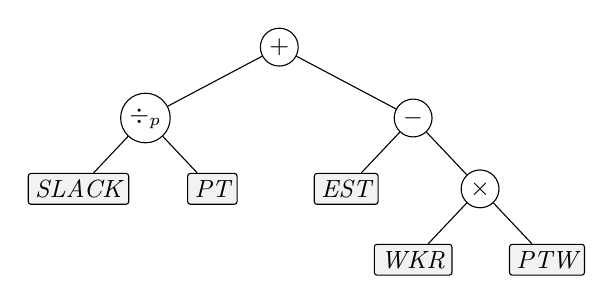
\begin{tikzpicture}[
  level distance=9mm,
  level 1/.style={sibling distance=34mm},
  level 2/.style={sibling distance=17mm},
  op/.style={circle, draw, inner sep=1.5pt, font=\small},
  term/.style={rectangle, draw, rounded corners=1pt, inner sep=2.5pt,
               font=\small\itshape, fill=black!5}]
\node[op] {$+$}
  child {node[op] {$\div_p$}
    child {node[term] {SLACK}}
    child {node[term] {PT}}}
  child {node[op] {$-$}
    child {node[term] {EST}}
    child {node[op] {$\times$}
      child {node[term] {WKR}}
      child {node[term] {PTW}}}};
\end{tikzpicture}
\caption{An individual is a priority expression tree; leaves are
interval-aware attributes of the candidate operation (here the
illustrative rule $\mathit{SLACK}/\mathit{PT} + \mathit{EST} -
\mathit{WKR}\cdot\mathit{PTW}$).}
\label{fig:tree}
\end{figure}

\subsection{Hyper-heuristic view: from expression trees to schedules}
\label{sec:hhview}
An individual is a priority expression tree (Figure~\ref{fig:tree}).
Leaves are drawn from the interval-aware terminal set of
Table~\ref{tab:terminals}. Its three \emph{width terminals},
$\mathit{PTW}$, $\mathit{ESTW}$ and $\mathit{WKRW}$, expose the widths of
the intervals. Internal nodes are drawn from the function set
\begin{equation}
\mathcal{F} = \{\, +,\; -,\; \times,\; \div_p,\; \min,\; \max,\;
\mathrm{neg} \,\},
\end{equation}
where $\mathrm{neg}$ is the unary sign change and $\div_p$ denotes
protected division, defined as $a \div_p b = a/b$ if $|b| > 10^{-9}$ and
$a$ otherwise.

The rule is deployed inside a semi-active schedule generation scheme
(SGS). Starting from the empty schedule, the SGS takes $n\,m$ decisions.
At each one it forms the set $\mathcal{E}$ of eligible operations, those
whose job predecessor is already scheduled, and evaluates the tree on
the attributes of every $o \in \mathcal{E}$. The operation with the
lowest priority value is appended at its earliest feasible start on its
machine, Eq.~\eqref{eq:sgs}. Ties are broken by the lowest job index, so
a rule maps each instance to exactly one schedule.

Because the lowest value is dispatched, a criterion that seeks to \emph{maximize}
an attribute must be expressed through the unary $\mathrm{neg}$
operator. Classic rules thus have counterparts in this search space: the
single-node tree $\mathit{PT}$ is shortest processing time on the upper
endpoints, and $\mathrm{neg}(\mathit{WKR})$ is most work remaining. They
differ from the SPT and MWKR baselines of Section~\ref{sec:reference}
only on ties, which the trees break by job index and the baselines by
the lower endpoint, Eq.~\eqref{eq:rank}. We inject both trees as seeded rules in the initial population.




\subsection{Evolutionary components}
\label{sec:evoview}
The initial population is built with the \emph{ramped half-and-half}
method~\citep{Koza1992,Poli2008}. Each individual draws its maximum
depth uniformly from $\{2,3,4\}$. With equal probability it is then
generated by the \emph{full} method, which expands every branch with
function nodes down to that depth, or by the \emph{grow} method, which
may close a branch earlier by placing a terminal, with probability
$0.3$ per node. In both cases internal nodes are drawn uniformly from
$\mathcal{F}$ and leaves uniformly from the terminal set. The last two members of the
population are not generated at random: they are the two seeded rules
of Section~\ref{sec:hhview}, inserted directly.
Every individual is evaluated by the mean $\RE$ of its
deterministic constructive pass over the four training instances.
The ranking of Eq.~\eqref{eq:rank} compares schedules of a single
instance, whereas fitness must summarize a rule over several, so it uses
the scalar $\RE$, the measure in which the IJSP literature reports its
results.

\begin{algorithm}[t]
\caption{GP hyper-heuristic for the IJSP}
\label{alg:gp}
\begin{algorithmic}[1]
\State $P \gets$ ramped half-and-half($\mathit{pop}-2$) $\cup$ \{$\mathit{PT}$, $\mathrm{neg}(\mathit{WKR})$\}
\State evaluate($P$) \Comment{mean RE of one constructive pass on the
training instances}
\For{$g = 1$ \textbf{to} $\mathit{gens}$}
  \State $P' \gets$ elite($P$, $e$) \Comment{elitism}
  \While{$|P'| < \mathit{pop}$}
    \If{rand() $< p_c$}
      \State $p_1, p_2 \gets$ tournament($P,k$), tournament($P,k$)
      \State $\mathit{child} \gets$ subtreeCrossover($p_1$, $p_2$)
    \Else
      \State $\mathit{child} \gets$ subtreeMutation(tournament($P,k$))
    \EndIf
    \State $P' \gets P' \cup \{\mathit{child}\}$ \Comment{fitness $\infty$ if
    size $> c$}
  \EndWhile
  \State $P \gets$ evaluate($P'$)
\EndFor
\State \Return best rule in $P$
\end{algorithmic}
\end{algorithm}

\begin{table}[t]
\centering\small
\caption{Evolution parameters: the configuration selected by irace
(Section~\ref{sec:irace}), used for every experiment reported in this
paper unless a section states otherwise.}
\label{tab:gpparams}
\begin{tabular}{ll}
\toprule
Population / generations & $100$ / $50$ \\
Initialization & ramped half-and-half (depths $2$--$4$) \\
Seeded individuals & $\mathit{PT}$ and $\mathrm{neg}(\mathit{WKR})$ \\
Selection & tournament, size $k = 7$ \\
Crossover / mutation prob. & $p_c = 0.77$ / $0.23$ (subtree, depth $\le 3$) \\
Elitism & $e = 2$ \\
Tree-size cap & $c = 30$ nodes (violations: fitness $\infty$) \\
Fitness & mean RE of one constructive pass, TA11--TA14 \\
Seeds & $1$--$30$ (random generator of the evolution) \\
\bottomrule
\end{tabular}
\end{table}

Each generation then proceeds as follows. Parents are chosen by
tournament, drawing $k$ individuals uniformly without replacement from
the current population and returning the fittest of them. With
probability $p_c$ two parents are recombined by \emph{subtree
crossover}~\citep{Koza1992,Poli2008}. A node is drawn uniformly at
random in each parent, leaves included. The offspring is a copy of the
first parent in which the subtree rooted at its chosen node is replaced
by the one rooted at the second parent's. Unlike the classical
two-offspring formulation, we keep a single offspring per recombination.
With the complementary probability, a single parent undergoes
\emph{subtree mutation}: a node is drawn uniformly at random, and the
subtree rooted at it is replaced by a random tree built with the grow
method and maximum depth $3$. Offspring whose size exceeds a cap of $c$
nodes receive infinite fitness and are thereby excluded from selection.
The depth bounds apply only to trees created from scratch, at
initialization and inside mutation. During the run only the node count
is bounded, so recombination may produce deeper expressions.

Replacement is fully generational, the offspring becoming the next
population, except for the $e$ best individuals of the current
generation, which are copied into it unchanged. The process stops after
a fixed number of generations and returns the best rule found.
Algorithm~\ref{alg:gp} summarizes the generational loop and
Table~\ref{tab:gpparams} lists the parameter values.


\subsection{Randomized multi-start extension}
\label{sec:grasp}
A deterministic rule produces one schedule. For comparisons with
sampling-based methods at matched budget, we wrap the evolved rule in
GRASP-style randomization~\citep{Feo1995}. With probability $0.1$ the
dispatched operation is drawn uniformly from the eligible set; otherwise
the rule decides. Sample $0$ remains deterministic. The wrapper, which
we call GP-best-of-$N$, reports the lexicographically best of its $N$
schedules. This uniform perturbation of a single rule is the simplest
member of a family of randomized rule-based builders; an alternative
swaps among a \emph{set} of evolved rules during
construction~\citep{GilGala2025GRASB}. GP-best-of-$N$ turns any budget
beyond a single pass into better schedules. As in GRASP, the gain comes
from sampling more schedules, not from better individual decisions. It
is compared with per-instance search in Sections~\ref{sec:metaheur}
and~\ref{sec:budget}.

\section{Experimental Setup}
\label{sec:setup}

\subsection{Benchmark instances and data split}
\label{sec:instances}
We use two benchmarks from the IJSP
literature~\citep{DiazGA2020,DiazFEABC2023,DiazICAE2023}. The first is
the 70 interval versions of Taillard's instances~\citep{Taillard1993}
(TA1--TA70), in seven size classes from $15{\times}15$ to $50{\times}20$.
The second is the 12 classical instances on which the published IJSP
metaheuristics report results: FT10 and FT20~\citep{FisherThompson1963},
seven instances of the La family~\citep{Lawrence1984} and
ABZ7--9~\citep{Adams1988}, with $10$ to $20$ jobs and $5$ to $15$
machines. Both were obtained from their crisp counterparts with the
generation scheme of \citet{DiazGA2020}. For every operation of original
duration $p$, a value $\delta$ is drawn uniformly at random in
$[0,\, 0.15\,p]$, and the duration becomes the integer interval
$[p-\delta,\, p+\delta]$. Machine routes are unchanged. The interval is
symmetric around $p$, so the crisp instance is exactly the midpoint
scenario of its interval version. Both sets are released with this
paper (see Data availability).

The 70 interval Taillard instances are split three ways. Rules are
evolved on TA11--TA14 ($20{\times}15$). TA15--TA20 form the
validation set: they never contribute to fitness, but the design and
configuration decisions of this paper, including the irace study of
Section~\ref{sec:irace}, were selected on their performance. The
remaining 60 instances play no part in any of these decisions. Together
with the 12 classical instances, to which the rules are applied without
re-evolution (Section~\ref{sec:classics}), they form the generalization
test.

Thirty independent evolutions, differing only in their random seed,
yield thirty rules. The one with the lowest mean $\RE$ on the validation
set is the \emph{featured rule}. Results are reported as the mean over
the 30 rules, which involves no selection, together with the value of
the featured rule. Where a section examines a single rule, it states how
that rule is chosen.

For the analysis of Section~\ref{sec:asym}, the 70 Taillard instances
were also regenerated with intervals skewed to the right. The crisp
duration $p$ is recovered from the midpoint of the symmetric version,
which the scheme above preserves exactly. The bounds are drawn as
$p - \mathrm{round}(p\,U[0,0.05])$ and
$p + \mathrm{round}(p\,U[0,0.25])$, so a duration may fall up to $5\%$
below its nominal value and up to $25\%$ above it. Machine routes are
unchanged, and the crisp Taillard bounds still apply. Over the
$37{,}250$ operations, the mean width is $14.3\%$ of $p$, against
$12.9\%$ for the symmetric scheme. The two benchmarks thus differ above
all in the shape of the intervals; the asymmetric ones are also wider,
by $1.4$ points of $p$ on average.


\subsection{Reference methods}
\label{sec:reference}
The constructive baselines are the dispatching rules of
Section~\ref{sec:related} (SPT, LPT, EST, MWKR, MOR and CR) and the two
Giffler--Thompson combinations, G\&T-SPT and G\&T-MWKR, each applied in
one deterministic pass. Each ranks candidates by its own criterion under
the lexicographic order of Eq.~\eqref{eq:rank}.
Section~\ref{sec:decoder} checks that this choice does not handicap
them. A dispatcher that chooses uniformly
among the eligible operations serves as a reference point.

The sampled variant of the evolved rule is GP-best-of-$N$
(Section~\ref{sec:grasp}). The published IJSP metaheuristics are
implemented in C\texttt{++} and report results under their own stopping
rules, which does not allow them to be compared with the evolved rule at
a matched budget. For that comparison we implemented our own version of
the genetic algorithm of \citet{DiazGA2020} in Python, on the decoder
and evaluator of Section~\ref{sec:problem}, so that it and the evolved
rule differ only in the method. A solution is a permutation with
repetition of jobs, decoded by the semi-active scheme of
Eq.~\eqref{eq:sgs} and compared by the ranking of Eq.~\eqref{eq:rank}.
A population of $250$ individuals is initialized at random. Parents are
chosen by tournaments of size $3$ and recombined with probability $0.9$
by a job-based order crossover: a random subset of jobs keeps its
positions from the first parent, and the remaining positions are filled
in the order they take in the second. Offspring are mutated with
probability $0.2$ by swapping two positions, and the two best
individuals pass unchanged to the next generation.

\subsection{Hyperparameter configuration with irace}
\label{sec:irace}
Four parameters of the evolution were configured with
irace~\citep{LopezIbanez2016}: tournament size, crossover probability,
tree-size cap and elitism. Population size and number of generations
were held fixed, so every configuration runs the same number of
evaluations. irace was given 200 experiments, each a full evolution on
the training instances scored by the validation $\RE$ of the resulting
rule. Table~\ref{tab:irace} lists the parameter space and the winning
configuration (Table~\ref{tab:gpparams}). Of the four elite
configurations that irace retains, three favor a high selection
pressure (tournament size $7$), and all four fall in a narrow crossover
band, $0.72$--$0.77$. The tree-size cap does not discriminate: the
elites span caps of $20$, $30$ and $40$.

\begin{table}[t]
\centering\small
\caption{Hyperparameter space explored by irace (200 experiments; cost =
validation-set RE of the evolved rule) and the winning configuration.}
\label{tab:irace}
\begin{tabular}{lcc}
\toprule
Parameter & Range / values & irace winner \\
\midrule
Tournament size & $\{2, 3, 4, 5, 7\}$ & $7$ \\
Crossover prob.\ $p_c$ & $[0.5,\, 0.95]$ & $0.77$ \\
Tree-size cap & $\{20, 30, 40, 60\}$ & $30$ \\
Elitism & $\{1, 2, 4\}$ & $2$ \\
\bottomrule
\end{tabular}
\end{table}


\subsection{Evaluation measures and statistical analysis}
\label{sec:stats}
Every measure below is to be minimized. Those that concern the
execution of a schedule are estimated by Monte Carlo over realizations
of the durations, as described in Section~\ref{sec:robustness}.
\begin{itemize}
\item \emph{Quality}: the relative error $\RE$ of
  Section~\ref{sec:problem}, in percent.
\item \emph{Width of the prediction}: the relative width of the interval
  makespan,
  $W = (\overline{C}_{\max}-\underline{C}_{\max})/E[\mathbf{C}_{\max}]
  \times 100$.
\item \emph{Executional robustness}: the mean deviation of the executed
  makespan from its prediction, relative to the expected makespan
  ($\bar\varepsilon$, Eq.~\eqref{eq:eps}) and in time units
  ($|\Delta|$, the same average before dividing by
  $E[\mathbf{C}_{\max}]$).
\item \emph{Tail of the execution}: the conditional value-at-risk at
  level $0.95$, $\mathrm{CVaR}_{0.95}$, the mean of the $5\%$
  largest values of a quantity over the same realizations. It is applied
  to the overrun $C^{\mathrm{ex}}_{\max}-E[\mathbf{C}_{\max}]$ of the
  executed makespan beyond its prediction, in time units, and to the
  executed makespan itself, expressed as $\RE$ over the same bound
  $\LB$.
\end{itemize}

Comparisons are of two kinds, with different experimental units.
Methods are compared instance by instance, pairing their values on the
same instances; when a method is run several times on each instance,
its value on an instance is the mean over the runs. The test is the
two-sided Wilcoxon signed-rank test with exact $p$-values, reported with
the normal-approximation statistic $z$ and, as effect size, the
matched-pairs rank-biserial correlation $|r|$. An \emph{arm} is a set of
evolutions, 30 unless stated otherwise, run with the same configuration
(terminal set, fitness and training instances) and differing only in the
random seed. The \emph{full} arm uses the complete terminal set, and the
\emph{ablated} one omits the width terminals. Two arms share nothing but
the seed numbers, so they are compared as independent samples of rules,
each rule averaged over the instances. The test is the two-sided
Mann--Whitney rank-sum test, reported with its normal-approximation $z$,
negative when the first arm named has the lower values. Its effect size
is the rank-biserial correlation $|r|$, which is $1$ when the two arms
do not overlap. In
Section~\ref{sec:budget}, whose many contrasts are each over 10 to 12
instances, the Wilcoxon test is reported instead with the number of
instances favoring each method. Holm's correction is applied within each family
of related comparisons, and where it changes a verdict the text says
so.

\subsection{Computing environment}
\label{sec:env}
All experiments ran on a desktop computer with an AMD Ryzen~5~3400G
processor (4 cores, 8 threads) and 32~GB of RAM under Windows~10~Pro.
The hyper-heuristic, the decoder, the baselines and the genetic
algorithm are implemented in Python~3.12 with NumPy~2.3, statistical
tests use SciPy~1.17, and the configuration study used
irace~4.4.3~\citep{LopezIbanez2016}. All reported times are wall-clock times of a single
simulator, which builds exactly the same schedules as the one used
during evolution. They were measured with six runs executing in
parallel, and are comparable with one another but not with times
obtained on other hardware or in other languages.

\section{Results}
\label{sec:results}


\subsection{Evolution behavior and seed stability}
Over 30 independent evolutions, training $\RE$ converges to
$14.9 \pm 1.5$ (range $12.4$--$19.7$), with most of the improvement
realized by generation $25$--$30$ (Figure~\ref{fig:convergence}a).
Each evolution takes about $26$~min ($24$--$28$ over the 30 seeds) on the
machine of Section~\ref{sec:env}, an offline cost paid once per rule.
The same panel evaluates the best rule of each generation on the
instances the fitness never sees, and there the improvement is
concentrated in the first ten generations. From generation $10$ to $50$
the median training $\RE$ falls from $17.09$ to $14.57$. On the $60$
test instances it falls only from $19.32$ to $18.71$, and on the
validation set it hardly moves, from $19.85$ to $19.69$. The later
generations thus specialize the rule to the four training instances more
than they improve it elsewhere, and the validation set could also serve
to stop the evolution earlier at a small cost in quality. Over the same
generations the best rules grow to a median of $27$ nodes, just below
the cap of $30$ (Figure~\ref{fig:convergence}b). Interval-width
terminals make up about a fifth of their leaves throughout
(Figure~\ref{fig:convergence}c).
Figure~\ref{fig:besttree}
shows the featured rule, obtained with seed~1: $26$ nodes
over $12$ leaves. Every terminal of the tree is non-negative by
construction and processing times are at least one time unit, so its
$\min$ and $\max$ nodes always select the same argument. On the
problem domain the tree is therefore exactly equivalent to the
expression
\begin{equation}
\mathit{SLACK}^{2} \;+\; 2\,\mathit{PT}
\;-\; \mathit{WKR} \;-\; \mathit{WKRW} \;-\; 1 .
\label{eq:besttree}
\end{equation}
We verified this identity at each of the $37{,}250$ dispatching decisions
the rule takes on the benchmark ($1.29$ million candidate evaluations).

\begin{figure}[t]
\centering
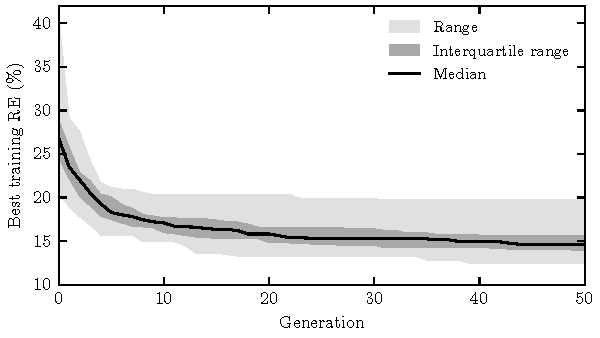
\includegraphics[width=\linewidth]{figures/fig_convergence.pdf}
\caption{The best rule of each generation over the 30 evolutions: (a) $\RE$ on
the training, validation and test instances, (b) size in nodes, (c)
share of interval-width terminals among its leaves. Lines are medians
(means in c); bands are interquartile ranges.}
\label{fig:convergence}
\end{figure}

\begin{figure}[t]
\centering
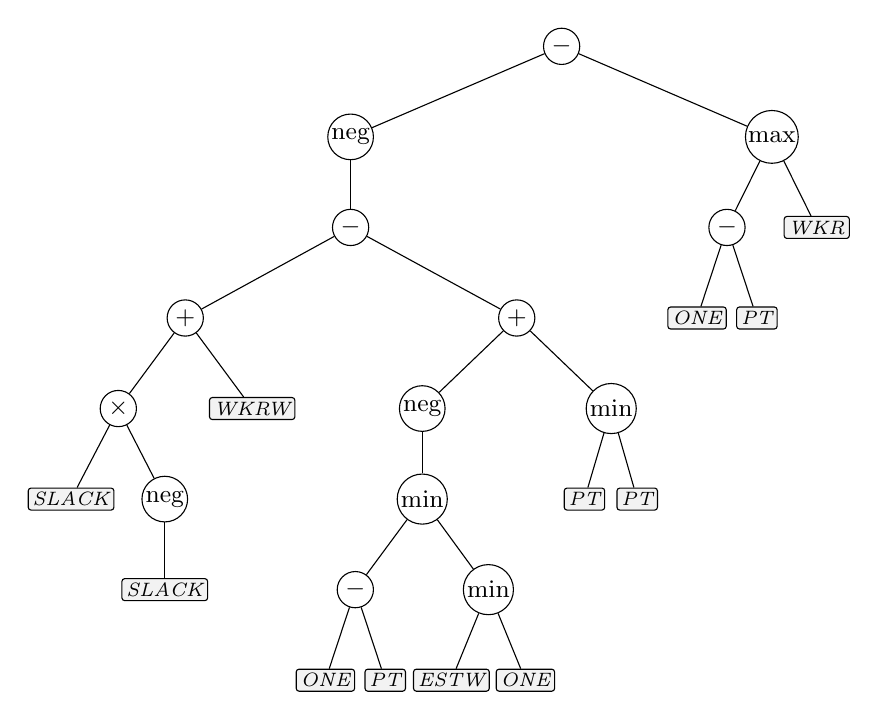
\begin{tikzpicture}[
  op/.style={circle, draw, inner sep=0.6pt, minimum size=4.6mm,
             font=\small},
  term/.style={rectangle, draw, rounded corners=1pt, inner sep=1.6pt,
               font=\scriptsize\itshape, fill=black!5}]
  \node[term] (n5) at (0.55,-5.75) {SLACK};
  \node[term] (n7) at (1.74,-6.90) {SLACK};
  \node[op] (n6) at (1.74,-5.75) {neg};
  \node[op] (n4) at (1.15,-4.60) {$\times$};
  \node[term] (n8) at (2.85,-4.60) {WKRW};
  \node[op] (n3) at (2.00,-3.45) {$+$};
  \node[term] (n13) at (3.78,-8.05) {ONE};
  \node[term] (n14) at (4.54,-8.05) {PT};
  \node[op] (n12) at (4.16,-6.90) {$-$};
  \node[term] (n16) at (5.38,-8.05) {ESTW};
  \node[term] (n17) at (6.32,-8.05) {ONE};
  \node[op] (n15) at (5.85,-6.90) {min};
  \node[op] (n11) at (5.01,-5.75) {min};
  \node[op] (n10) at (5.01,-4.60) {neg};
  \node[term] (n19) at (7.07,-5.75) {PT};
  \node[term] (n20) at (7.74,-5.75) {PT};
  \node[op] (n18) at (7.41,-4.60) {min};
  \node[op] (n9) at (6.21,-3.45) {$+$};
  \node[op] (n2) at (4.10,-2.30) {$-$};
  \node[op] (n1) at (4.10,-1.15) {neg};
  \node[term] (n23) at (8.50,-3.45) {ONE};
  \node[term] (n24) at (9.26,-3.45) {PT};
  \node[op] (n22) at (8.88,-2.30) {$-$};
  \node[term] (n25) at (10.02,-2.30) {WKR};
  \node[op] (n21) at (9.45,-1.15) {max};
  \node[op] (n0) at (6.78,0.00) {$-$};
  \draw (n6) -- (n7);
  \draw (n4) -- (n5);
  \draw (n4) -- (n6);
  \draw (n3) -- (n4);
  \draw (n3) -- (n8);
  \draw (n12) -- (n13);
  \draw (n12) -- (n14);
  \draw (n15) -- (n16);
  \draw (n15) -- (n17);
  \draw (n11) -- (n12);
  \draw (n11) -- (n15);
  \draw (n10) -- (n11);
  \draw (n18) -- (n19);
  \draw (n18) -- (n20);
  \draw (n9) -- (n10);
  \draw (n9) -- (n18);
  \draw (n2) -- (n3);
  \draw (n2) -- (n9);
  \draw (n1) -- (n2);
  \draw (n22) -- (n23);
  \draw (n22) -- (n24);
  \draw (n21) -- (n22);
  \draw (n21) -- (n25);
  \draw (n0) -- (n1);
  \draw (n0) -- (n21);
\end{tikzpicture}

\caption{The featured rule (seed~1) as evolved; shaded boxes are the terminals
of Table~\ref{tab:terminals}, and Eq.~\eqref{eq:besttree} gives its
simplified form.}
\label{fig:besttree}
\end{figure}


\subsection{Position among constructive methods}
\label{sec:baselines}
Table~\ref{tab:baselines} reports every constructive baseline under the
protocol of this paper, one deterministic pass per instance, together
with the random dispatcher of Section~\ref{sec:reference}. Since these rules are
deterministic, the standard deviation is taken across instances: it
measures how uniform a method is over the benchmark, not any run-to-run
variability. The random dispatcher, the one stochastic entry, is
averaged over 10 dispatches per instance. Times are averages over
the 70 instances with 5 repetitions each. The GP entries are the
featured rule, timed as evolved, and the same rule in its simplified
form, which takes the same decisions.

Two observations are needed to read the table correctly. First, the
plain rules that ignore machine availability, SPT, LPT and the critical
ratio CR, perform \emph{worse than random} in this setting; CR is a
due-date rule, applied here without due dates. This is a
property of the schedule generation scheme, not a defect of the
criteria: because a solution is decoded as a permutation whose
operations are appended to their machines, systematically dispatching
by processing time alone produces highly unbalanced permutations. The
same criterion embedded in the Giffler--Thompson conflict set, which
restores classical dispatching semantics, behaves as expected
(SPT: $627\%$ as a plain rule versus $70.6\%$ under G\&T). Second, the
criteria that do account for the state of the shop (EST, MOR, MWKR) are
better than random, and the strongest baseline overall is
G\&T-MWKR at $29.5\%$, which is the reference we use throughout.

Against that strongest baseline, the 30 evolved rules average
$18.99 \pm 1.33$ $\RE$, and the featured rule attains $17.71\%$, the
lowest of the 30 on these instances although it was selected on the
validation set.

\begin{table}[t]
\centering\small
\caption{Constructive baselines on the 70 interval Taillard instances: mean RE
(\%), standard deviation across instances, and time of one pass (ms), all
on the same simulator.}
\label{tab:baselines}
\begin{tabular}{lccc}
\toprule
Method & RE (\%) & sd & Time (ms) \\
\midrule
LPT & 703.6 & 168.0 & 4.2 \\
SPT & 627.2 & 152.2 & 4.2 \\
CR & 625.7 & 140.6 & 3.3 \\
\midrule
\textit{Random dispatcher} & \textit{127.2} & \textit{13.9} & \textit{1.1} \\
\midrule
G\&T-SPT & 70.6 & 10.0 & 14.3 \\
MWKR & 64.7 & 10.4 & 5.0 \\
MOR & 45.5 & 10.1 & 2.7 \\
EST & 42.3 & 10.6 & 9.8 \\
G\&T-MWKR & \textbf{29.5} & 6.4 & 17.4 \\
\midrule
GP rule (featured) & \textbf{17.71} & 5.23 & 20.6 \\
\quad simplified, Eq.~\eqref{eq:besttree} & 17.71 & 5.23 & 11.1 \\
\bottomrule
\end{tabular}
\end{table}
The gap holds on every instance: the featured rule outperforms each of
the eight deterministic baselines on all $70$, and a paired Wilcoxon
signed-rank test rejects equality against each of them at $p<10^{-6}$
($z=-7.3$), also after Holm's correction for the eight comparisons. The
narrowest margin over the whole comparison is $3.9$ points, against
G\&T-MWKR on a single $20{\times}15$ instance. Against the best plain
rule, EST, the smallest margin is $6.3$ points. Per-instance figures are given in
Supplementary Table~\ref{S-tab:perinstance}. This quality comes at
a small evaluation cost. A pass of the featured rule takes
$20.6$~ms as evolved and $11.1$~ms in its simplified form,
against $17.4$~ms for G\&T-MWKR, the strongest baseline, and
$2.7$~ms for MOR, which reads a single attribute.

\subsection{Generalization across sizes and instance families}
\label{sec:generalization}
\label{sec:classics}
Table~\ref{tab:gp70} reports single-pass $\RE$ per size class over all
70 instances, as mean $\pm$ standard deviation across the 30 evolved
rules and for the featured rule. Evolved only on $20{\times}15$,
the featured rule attains its lowest $\RE$ on the
unseen $50{\times}15$ ($13.8\%$), and the same pattern holds on
average ($13.7 \pm 1.5$). Because all terminals are per-operation
attributes with no size-bound quantities, transfer requires no
retraining or rescaling.

The ranking of the classes reflects the difficulty of their instances
more than their distance from the training size. In the two 50-job
classes, where the rule does best, every crisp counterpart has been
solved to optimality~\citep{CoupventdesGraviers2025}. The bounds used
here equal the optimal makespans, so on these classes $\RE$ is measured
against the optimum. The error is largest on
$30{\times}20$, the class with the most open instances, nine of ten.
The reference bound of an open instance lies below its unknown optimum,
so part of the error measured there belongs to the bound: the best known
solutions of that class exceed the bounds used here by $2.7\%$ on
average.

\begin{table}[t]
\centering\small
\caption{RE (\%) per size class over the 70 interval Taillard instances: mean
$\pm$ sd of the 30 evolved rules, and the featured rule.}
\label{tab:gp70}
% 9 columnas = 18 huecos, asi que cada punto de tabcolsep vale 18pt de ancho:
% a 3.5pt la tabla medía 373.7pt contra los 360pt de \linewidth; con la
% etiqueta "Featured rule", a 2.5pt sobraban 3.9pt
\setlength{\tabcolsep}{2.2pt}
\scriptsize
\begin{tabular}{lccccccc|c}
\toprule
& $15{\times}15$ & $20{\times}15$ & $20{\times}20$ &
$30{\times}15$ & $30{\times}20$ & $50{\times}15$ & $50{\times}20$ & All \\
\midrule
Mean of 30 & $18.1{\pm}1.3$ & $18.0{\pm}1.5$ & $20.9{\pm}1.7$ &
$21.4{\pm}1.7$ & $25.7{\pm}1.9$ & $13.7{\pm}1.5$ & $15.1{\pm}1.5$ &
$18.99{\pm}1.33$ \\
Featured rule & 15.7 & 16.6 & 18.1 & 21.1 & 24.1 & \textbf{13.8} & 14.6 &
\textbf{17.71} \\
\bottomrule
\end{tabular}
\end{table}


The rules also transfer to the second benchmark, whose 12 classical
instances differ from the Taillard ones in origin, size and
structure.
Table~\ref{tab:classics} gives the featured rule's single-pass $\RE$ on
each, together with GP-best-of-$N$ at $N = 64$ and $N = 1024$ (GP-64 and
GP-1024) and the
published results of the IJSP metaheuristics, which
Section~\ref{sec:metaheur} discusses.

\begin{table}[t]
\centering\small
\caption{RE (\%) on the 12 classical interval instances: our methods and the
published averages over 30 runs per instance of GA~\citep{DiazGA2020},
ABC$_{E3}$~\citep{DiazABC2022}, fEABC~\citep{DiazFEABC2023} and
ESABC~\citep{DiazICAE2023}. LB is the reference bound of
Section~\ref{sec:problem}; GP-64 and GP-1024 are GP-best-of-$N$ with
$N = 64$ and $1024$.}
\label{tab:classics}
\setlength{\tabcolsep}{4.5pt}
\begin{tabular}{lrrrrrrrrr}
\toprule
& & & \multicolumn{3}{c}{Ours (zero-shot)} &
\multicolumn{4}{c}{Published (avg of 30)} \\
\cmidrule(lr){4-6}\cmidrule(l){7-10}
Inst. & LB & & GP & GP-64 & GP-1024 &
GA & ABC$_{E3}$ & fEABC & ESABC \\
\midrule
FT10 & 930 & & 20.4 & 8.4 & 6.6 & 5.2 & 4.1 & 3.5 & 3.0 \\
FT20 & 1165 & & 13.2 & 12.1 & 10.8 & 4.4 & 1.7 & 1.8 & 1.8 \\
La21 & 1046 & & 15.0 & 14.4 & 9.0 & 5.0 & 5.0 & 4.2 & 4.0 \\
La24 & 935 & & 10.1 & 8.8 & 8.6 & 6.3 & 5.1 & 4.9 & 5.0 \\
La25 & 977 & & 11.8 & 11.6 & 7.6 & 5.1 & 3.9 & 3.4 & 2.7 \\
La27 & 1235 & & 25.0 & 13.7 & 11.3 & 10.2 & 4.7 & 4.6 & 4.1 \\
La29 & 1152 & & 13.4 & 14.2 & 11.0 & 14.2 & 8.6 & 7.4 & 7.0 \\
La38 & 1196 & & 15.0 & 13.3 & 9.4 & 9.2 & 6.9 & 6.1 & 5.8 \\
La40 & 1222 & & 13.3 & 12.8 & 9.9 & 8.7 & 4.2 & 4.6 & 4.1 \\
ABZ7 & 656 & & 19.7 & 14.3 & 11.7 & 12.5 & 7.3 & 6.6 & 6.7 \\
ABZ8 & 645 & & 24.7 & 22.1 & 17.7 & 18.5 & 12.1 & 11.1 & 10.9 \\
ABZ9 & 661 & & 33.4 & 25.3 & 22.1 & 18.0 & 13.1 & 11.6 & 11.2 \\
\midrule
Mean & & & 17.9 & 14.2 & 11.3 & 9.8 & 6.4 & 5.8 & 5.5 \\
\bottomrule
\end{tabular}
\end{table}

Transfer is a property of the method rather than of one rule: over the
30 evolved rules the deterministic pass averages $19.04 \pm 1.97\%$
$\RE$ on these instances, single rules ranging from $15.3\%$ to
$23.3\%$. Since the two benchmarks use different reference bounds
(Section~\ref{sec:problem}), $\RE$ values do not compare across them,
but margins over baselines evaluated on the same instances do. That
margin is preserved: $2.40$ times over MOR and $1.58$ over G\&T-MWKR on
the classical set, against $2.40$ and $1.55$ on the benchmark the rules
were evolved for.

\subsection{Comparison with published metaheuristics}
\label{sec:metaheur}
On the 12 classical instances the evolved rules can be compared with the
published results of the IJSP metaheuristics on their own benchmark and
metric (Table~\ref{tab:classics}). Those methods belong to different
algorithmic families, evolutionary computation and swarm intelligence:
a genetic algorithm evolving a population of
permutations~\citep{DiazGA2020} and three artificial bee colony
variants~\citep{DiazABC2022,DiazFEABC2023,DiazICAE2023}, each of which runs a
separate search on every instance.

In a single pass the evolved rules average $19.04\%$ on these
instances, against $30.1\%$ (G\&T-MWKR) and $45.8\%$ (MOR) for the
deterministic baselines. With a $1024$-sample budget the featured rule
reaches $11.3\%$, within $1.5$ points of the $9.8\%$ published for the
genetic algorithm, which searches every instance separately. It is
better than the genetic algorithm on $3$ of the $12$ instances (paired
Wilcoxon $z = 1.96$, $p \approx 0.05$). The ABC variants, which add neighborhood structures
and local search to the population, remain ahead ($5.5$--$6.4\%$), as
expected of purpose-built iterative search. The comparison thus places
the evolved rules at the frontier of constructive methods, close to a
plain population-based search.

The two families also differ in how they spend computation:
GP-1024 evaluates $1024$ mutually independent samples per instance,
which can run in parallel, whereas the metaheuristics evolve a
population of $250$ individuals~\citep{DiazGA2020,DiazFEABC2023} through
successive generations, each of which depends on the previous one.

\subsection{Comparison at matched budget with a reimplemented genetic
algorithm}
\label{sec:budget}
For a comparison at matched budget we implement the genetic algorithm of
\citet{DiazGA2020} (Section~\ref{sec:reference}) in Python; its
implementation is included in the data repository (see Data
availability). On the 12
classical instances it achieves $7.3\%$ $\RE$ in $900$~s per instance,
against the $9.8\%$ published for the original, whose runs are
shorter. The rule and the genetic
algorithm share decoder, evaluator and language. The seeded genetic
algorithm places the permutation built by one pass of the featured rule
in its initial population, alongside $249$ random ones. The comparison is run
on the 12 classical instances, with 30 runs of $900$~s per instance and
method, and on three Taillard classes representative of the different
instance sizes, $15{\times}15$, $30{\times}15$ and $50{\times}15$. Each method is run 3 times on each of
the 10 instances of a class, for a total of 30 runs per class. The
horizons are $900$, $1800$ and $3600$~s per instance, chosen to extend
well beyond the point where the curves converge
(Figure~\ref{fig:budget}).

\begin{figure}[t]
\centering
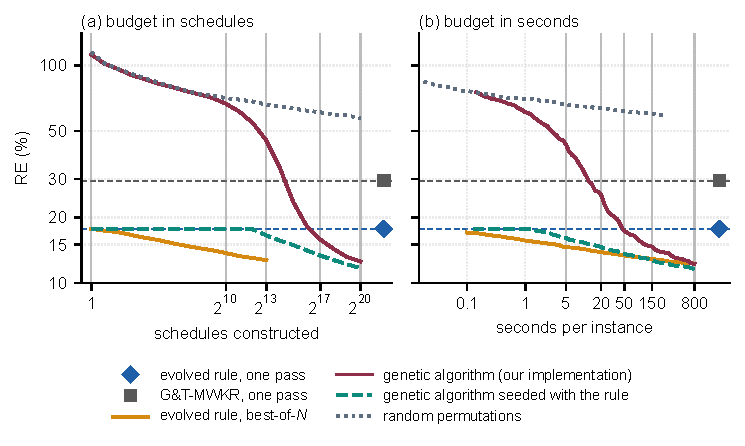
\includegraphics[width=\linewidth]{figures/fig_budget.pdf}
\caption{Mean RE of the best schedule found, over runs and instances,
against seconds per instance on the 12 classical instances (a) and on three Taillard classes with 15 machines, $15{\times}15$ (b),
$30{\times}15$ (c) and $50{\times}15$ (d).}
\label{fig:budget}
\end{figure}

At low budgets GP-best-of-$N$ attains the lowest $\RE$ of all methods,
until the genetic algorithm surpasses it. The budget at which this
occurs increases with instance size, from approximately $10$~s per
instance on the classical instances and $25$~s on $15{\times}15$ to
approximately $300$~s on $50{\times}15$, with $83$~s on the
intermediate $30{\times}15$ class. The rule is therefore the most
effective method at low budgets, a regime that extends further the
larger the instance. Seeding the genetic algorithm with the featured rule
likewise yields an initial advantage over the unseeded version, but the
two converge: from $100$~s per instance onwards, the statistical tests
detect no difference between them on any instance set (Supplementary
Table~\ref{S-tab:semilla}). An evolved dispatching rule thus delivers in
a single pass of milliseconds a quality that the genetic algorithm
needs between $2$ and $46$~s per instance to reach. As a seed, it gives
a population-based method a high-quality initial solution from which
the search progresses faster, the role constructive heuristics commonly
play in the initialization of such methods~\citep{Kazimipour2014}.

\section{Analysis}
\label{sec:analysis}



\begin{figure}[!t]
\centering
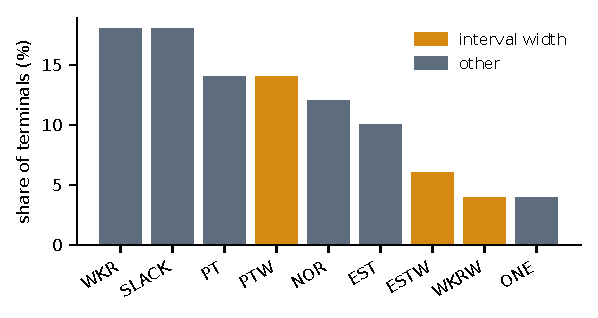
\includegraphics[width=.8\linewidth]{figures/fig_terminals.pdf}
\caption{Terminal usage across the 30 evolved rules, as a share of all
terminals; interval-width terminals in amber.}
\label{fig:terminals}
\end{figure}

\begin{figure}[!t]
\centering
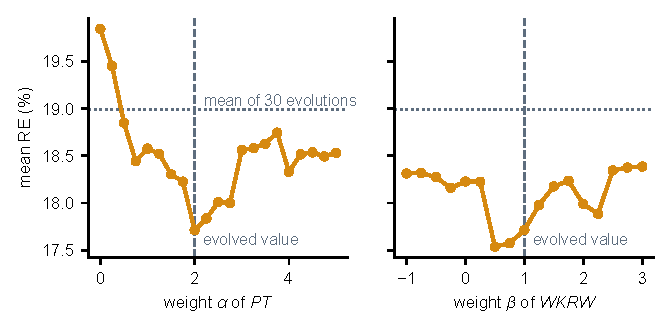
\includegraphics[width=.9\linewidth]{figures/fig_sensitivity.pdf}
\caption{Mean $\RE$ of the featured rule over the 70 instances as each weight of
its simplified form, Eq.~\eqref{eq:besttree}, varies with the other
fixed. Dashed lines: evolved weights; dotted line: mean of the 30
evolved rules; $\beta = 0$ removes the width term.}
\label{fig:sensitivity}
\end{figure}

\subsection{Rule anatomy and interpretability}
\label{sec:anatomy}
The output of GP is a readable expression. Evolved rules are compact,
with a mean tree size of $26$ nodes ($20$--$30$) and mean depth $9$, so
a rule can be inspected and simplified by hand.
Figure~\ref{fig:terminals} reports how often each terminal is used
across the 30 evolved rules. The most frequent are the classical
scheduling attributes, slack ($\mathit{SLACK}$), work remaining
($\mathit{WKR}$) and earliest start ($\mathit{EST}$), together with
worst-case processing time ($\mathit{PT}$): the evolution builds on
known dispatching logic. The \emph{interval-width} terminals ($\mathit{PTW}$,
$\mathit{ESTW}$, $\mathit{WKRW}$) account for $21.7\%$ of all
terminal usage and appear in $27$ of the $30$ evolved rules. Whether
that width information translates into better schedules is quantified in
Sections~\ref{sec:ablation}--\ref{sec:robustness}.

Since the lowest value is dispatched, the featured rule,
Eq.~\eqref{eq:besttree}, reads directly: $-\mathit{WKR}$ is most-work-remaining, $2\,
\mathit{PT}$ is shortest-processing-time at double weight, $\mathit{
SLACK}^{2}$ penalizes quadratically any operation that cannot start at
the earliest available time, and the constant is immaterial to the
ranking. The remaining term, $-\mathit{WKRW}$, is the interval-aware
one. Among jobs with comparable remaining work, the rule advances those
whose remaining work is \emph{more uncertain}, so that this uncertainty
is resolved early rather than carried to the end of the schedule; the
worked example of Section~\ref{sec:case} illustrates it.
The evolved rule is thus a weighted blend of MWKR and SPT, regularized
by a quadratic earliest-start term and tilted by the uncertainty of the
work ahead.

The simplified form of the featured rule, Eq.~\eqref{eq:besttree}, also
admits a direct sensitivity analysis: it weighs $\mathit{PT}$ by
$\alpha = 2$ and $\mathit{WKRW}$ by $\beta = 1$, and we swept each
weight over the 70 instances holding the other at its evolved value
(Figure~\ref{fig:sensitivity}). Neither curve is unimodal: over the
sampled grid, $\alpha$ has five local minima and $\beta$ three. Each
point is a deterministic evaluation over the 70 instances, so this
ruggedness belongs to the landscape, not to sampling noise. The evolved
$\alpha = 2$ is the global minimum of its sweep. The evolved $\beta$ is
not: it gives $17.71\%$, against $17.54\%$ for $\beta = 0.5$. A post-evolution weight sweep on the validation set is thus a cheap
refinement for any simplified rule. The multimodality becomes relevant if the sweep is replaced by local descent: started at $\alpha = 4$, a descent converges to a secondary minimum $0.6$ points above the global one. Setting
$\beta = 0$ removes the width term from the deployed rule and costs
$0.5$ points of $\RE$ ($18.23$ against $17.71$).


\subsection{A worked example}
\label{sec:case}

The example compares the rule with its variant without the width term
($\beta = 0$ in Section~\ref{sec:anatomy}) on a small instance with
three jobs of three operations. $J_1$ visits
$M_3, M_2, M_1$ with durations $[28,30]$, $[20,26]$, $[24,32]$; $J_2$
visits $M_1, M_3, M_2$ with $[26,30]$, $[10,12]$, $[16,18]$; and $J_3$
visits $M_3, M_1, M_2$ with $[22,26]$, $[14,14]$, $[27,31]$.

The two traces, that is, the sequences of dispatching decisions,
coincide in the first two decisions. They diverge at the third, where
$M_3$ has just been released by $o_{11}$ and the eligible set is
$\{o_{12}, o_{22}, o_{31}\}$. Table~\ref{tab:case} gives the
terminals and the resulting scores. All three candidates can start at
the same time, so SLACK vanishes and the decision rests on the
remaining terms. Without the width term the ranking puts $o_{22}$
($5$) ahead of $o_{31}$ ($6$): the short operation of the job with little work remaining ranks first because of the $2\,\mathit{PT}$ term. The width term contributes
$-\mathit{WKRW}$, which is $-4$ for $o_{31}$ against $-2$ for $o_{22}$,
and that reverses a one-point gap. The rule therefore dispatches
$o_{31}$, whose job has more uncertain remaining work than that of
$o_{22}$, $[41,45]$ against $[16,18]$. In this same state, SPT would
dispatch $o_{22}$ and MWKR $o_{31}$.

\begin{table}[t]
\centering\small
\caption{Terminals and priority scores at the third dispatching
decision of the worked example.}
\label{tab:case}
\begin{tabular}{lcccccc}
\toprule
Eligible & Duration & WKR & WKRW & SLACK & Eq.~\eqref{eq:besttree} &
$\beta = 0$ \\
\midrule
$o_{12}$ & $[20,26]$ & 32 & 8 & 0 & 11 & 19 \\
$o_{22}$ & $[10,12]$ & 18 & 2 & 0 & 3 & \underline{5} \\
$o_{31}$ & $[22,26]$ & 45 & 4 & 0 & \underline{2} & 6 \\
\bottomrule
\end{tabular}
\end{table}

\begin{figure}[t]
\centering
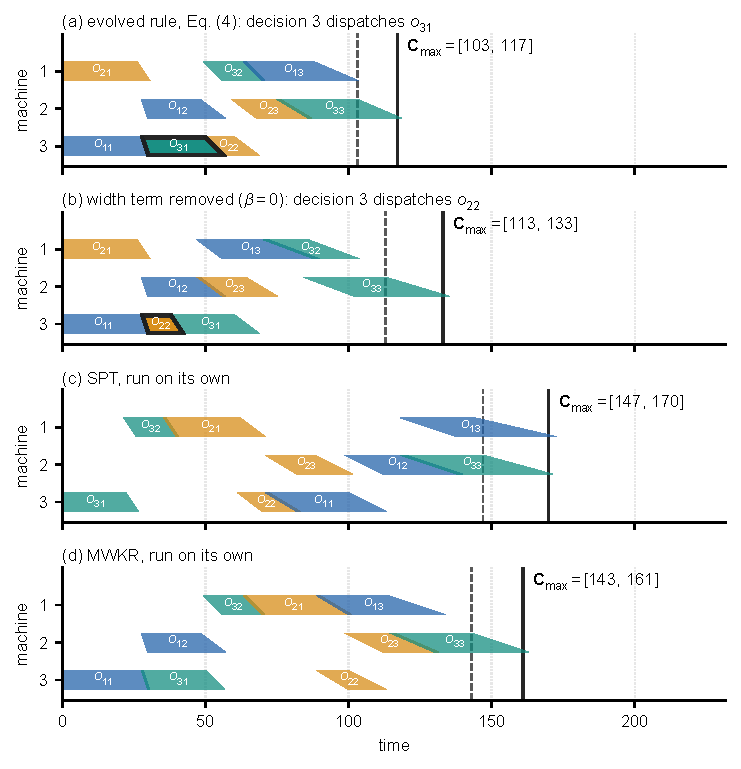
\includegraphics[width=\linewidth]{figures/fig_case.pdf}
\caption{The worked example scheduled by (a) the evolved rule, (b) the rule
without the width term, (c) SPT and (d) MWKR. The outlined operation
separates traces (a) and (b).}
\label{fig:case}
\end{figure}

Figure~\ref{fig:case} shows what follows. Dispatching $J_3$ early schedules its remaining operations
while the machines are still available, and the makespan is
$\mathbf{C}_{\max} = [103,117]$. Delaying it by that single decision
postpones the same operations to the end of the schedule, and the
makespan becomes $[113,133]$, worse at both endpoints. Run on their own
from the empty schedule (Figure~\ref{fig:case}c and~d), SPT and MWKR
yield $[147,170]$ and $[143,161]$, against a lower bound of $[72,88]$
set by the total work of $J_1$. Neither looks at when a candidate can
start, and the decoder appends each operation after the last one on its
machine. MWKR, which already departs from the evolved rule at the second
decision, dispatches $o_{32}$ before $o_{21}$ and leaves $M_1$ idle until
$[50,56]$. As a result $o_{21}$, which could have started at time $0$,
starts at $[64,70]$. SPT leaves $M_3$ idle from $[22,26]$ to $[62,70]$
in the same way. The $\mathit{SLACK}^2$ term of the evolved rule penalizes a candidate by how much later it would start than the earliest one.

The example illustrates the mechanism, not its magnitude. Over $800$
random $3{\times}3$ instances generated with the scheme of
Section~\ref{sec:instances}, removing the width term leaves the trace
unchanged in $668$. Of the $132$ traces that do change, $93$ end at the
same makespan, $21$ end better with the term and $18$ worse. Its
contribution over the 70-instance benchmark is measured in
Sections~\ref{sec:ablation} and~\ref{sec:robustness}.

\subsection{Interval handling and the decoder}
\label{sec:decoder}

The comparison with the constructive baselines could depend on two
choices that are not part of the rules themselves, and Supplementary
Section~\ref{S-sec:decoder} examines both. The first is how a baseline
compares intervals. Table~\ref{tab:baselines} ranks candidates
lexicographically, Eq.~\eqref{eq:rank}; ranking them instead by the
lower endpoint, the midpoint or the upper endpoint changes the $\RE$ of
EST and MWKR by at most $2.4$ points. That is far less than the $23.3$
points that separate the best of them, EST, from the evolved rules. The second
is the decoder. The evolved rules choose among all eligible operations
and build semi-active schedules, whereas G\&T-MWKR, the strongest
baseline, chooses only within Giffler and Thompson's conflict set and
builds active ones. Exchanging the decoders shows that the evolved rules
outperform MWKR under both: $18.99$ against $64.7$ with the semi-active
decoder and $23.18$ against $29.5$ with the conflict set. Each method in
Table~\ref{tab:baselines} is therefore reported with the decoder that
suits it, and the margin of the evolved rules does not depend on that
choice.

\subsection{The value of interval awareness: ablations}
\label{sec:ablation}
The interval-width terminals are the distinctive ingredient of this
setting, so we isolate their contribution by ablation. The 30
evolutions are repeated without the width terminals ($\mathit{PTW}$,
$\mathit{ESTW}$, $\mathit{WKRW}$), with everything else held fixed,
including the irace configuration of Section~\ref{sec:irace}. Interval information also enters the
evolution through the fitness, which scores every schedule by interval
arithmetic. To remove it as well, 30 further rules are evolved on the
crisp midpoint counterparts of the training instances
(Section~\ref{sec:instances}), with the same configuration and reduced
terminal set, so that they never handle interval data.
Figure~\ref{fig:ablation} shows the 30 rules of each arm, compared as
independent samples (Section~\ref{sec:stats}).
Supplementary Table~\ref{S-tab:ablation} gives their means; Holm's
correction over its tests changes none of the verdicts.

\begin{figure}[t]
\centering
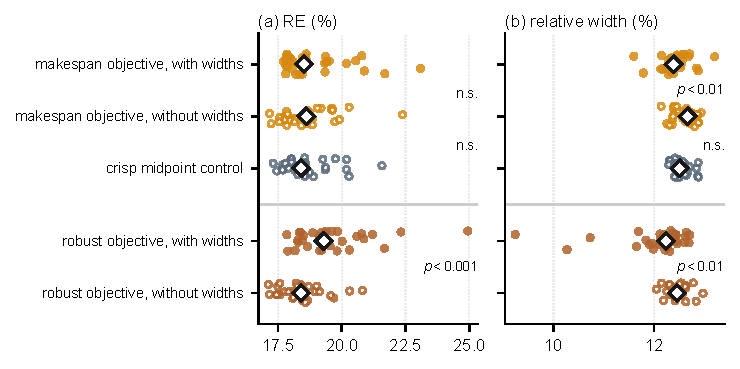
\includegraphics[width=\linewidth]{figures/fig_ablation.pdf}
\caption{The 30 evolved rules of each ablation arm, each averaged over the 70
instances: $\RE$ (a) and relative width of the predicted makespan
interval (b). Diamonds: medians; labels: Mann--Whitney test between
adjacent arms.}
\label{fig:ablation}
\end{figure}

The width terminals change the schedules even when nothing rewards it:
under the makespan objective, the rules that read them predict narrower
makespan intervals ($z=-2.96$, $p<0.01$,
$|r|=0.44$). In expected makespan, the quantity this objective
optimizes, the evolution reaches the same quality with or without them
(medians $18.52$ and $18.61$; $z=0.67$, n.s.). The crisp midpoint
control matches the interval-trained arm on both measures ($z=-0.12$ and
$z=-1.26$, n.s.), although the two fitness functions differ, since
$\max$ does not commute with taking midpoints. What
interval awareness adds is therefore not a lower expected makespan but
control over the width of the prediction, which
Section~\ref{sec:frontier} examines under an objective that rewards it.

\subsection{The robust objective: trading expected makespan for
predictability}
\label{sec:frontier}
The makespan fitness gives the evolution no incentive to trade expected
makespan for predictability. To test whether it can make that trade
when rewarded for it, we repeat the terminal ablation with a
\emph{robust} fitness that explicitly rewards predictability, minimizing
\begin{equation}
f_{\lambda} = \overline{C}_{\max} + \lambda\,
\big(\overline{C}_{\max}-\underline{C}_{\max}\big).
\label{eq:robustfit}
\end{equation}
The fitness rewards a low worst case \emph{and} a narrow interval, and
the weight $\lambda$ sets the balance between the two. Here
$\lambda = 1$, and the two bottom rows of Figure~\ref{fig:ablation} show
the outcome. Under this objective, the difference in width between the
arms with and without the width terminals doubles, from $0.20$ points
under the makespan objective to $0.42$. Rules evolved with the width
terminals produce significantly narrower makespan intervals
($12.04 \pm 0.75$ versus $12.47 \pm 0.20$ relative width;
Mann--Whitney $z=-2.99$, $p<0.01$, $|r|=0.45$). In exchange, their
expected makespan is higher ($19.62$ versus $18.42$ $\RE$; $z=3.59$,
$p<0.001$, $|r|=0.54$), which is the trade-off the robust objective is
designed to make.

\begin{figure}[t]
\centering
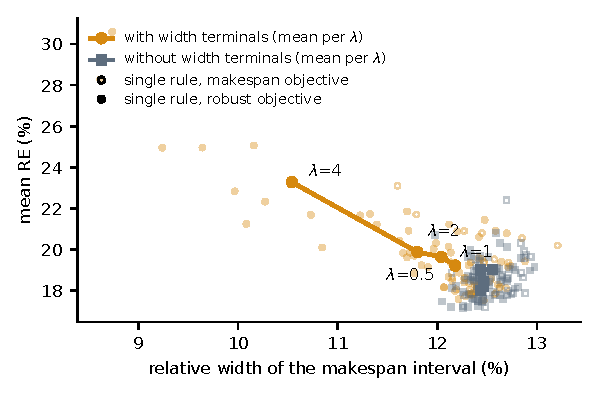
\includegraphics[width=.8\linewidth]{figures/fig_lambda.pdf}
\caption{Quality--predictability plane over the 70 instances. Faint markers are
evolved rules (amber with width terminals, grey without; open for the
makespan objective, filled for the robust one); curves join the arm
means along the $\lambda$ sweep of Eq.~\eqref{eq:robustfit}. The five
means without width terminals fall within $0.12$ points of width and are
unlabeled.}
\label{fig:lambda}
\end{figure}

The weight $\lambda$ of Eq.~\eqref{eq:robustfit} governs that trade-off,
and sweeping it traces the frontier between quality and predictability
(Figure~\ref{fig:lambda}). Both quantities move monotonically with
$\lambda$: as the weight grows from $0.5$ to $4$, the relative width of
the makespan interval falls from $12.18 \pm 0.50$ to
$10.54 \pm 1.26$ while the expected makespan degrades from
$19.20 \pm 1.52$ to $23.27 \pm 3.80$ $\RE$. At the far end of the sweep
the schedules are therefore narrower than any the ablated rules produced,
at a cost of about four points of $\RE$.

Sweeping $\lambda$ for the ablated arm (ten evolutions per value)
shows that it has no such curve. Its width stays between $12.43$ and
$12.56$ for every $\lambda$ from $0$ to $4$, and no individual rule
departs from this band, whereas the full arm goes from $12.18$ to
$10.54$. Penalizing width in the fitness therefore yields narrower
intervals only when the rule has terminals through which to act on it:
the objective works through the representation.

Read at the level of the arm, the price of narrowness rises along the
sweep. Between $\lambda = 2$ and $\lambda = 4$ the spread between
evolutions more than doubles, from $1.74$ to $3.80$, so the outcome of a
single run becomes much less predictable. A weight between $1$ and $2$
is therefore the default we would recommend. Selecting a rule within an
arm amplifies both sides of the trade-off: the narrowest rule of the
$\lambda = 1$ arm on the validation set, used in
Section~\ref{sec:robustness}, reduces $\bar\varepsilon$ by about a fifth
at a cost of $7.2$ points of $\RE$ with respect to the featured rule. For expected makespan alone the smaller
terminal set suffices (Section~\ref{sec:ablation}); the width terminals
become necessary when predictability matters.


\begin{table}[t]
\centering\small
\setlength{\tabcolsep}{4pt}
\caption{Predicted quality and executional robustness over the 70 instances:
$\RE$, relative width of the predicted interval, $\bar\varepsilon$
($\times10^3$) at nominal widths and widened by $+20\%$ and $+40\%$, and
$|\Delta|$ at nominal widths. Representatives: the featured rule; for
the robust arms, the narrowest rule on the validation set; for the
ablated arms, the best rule on the 70 instances, which favors them.
Supplementary Section~\ref{S-sec:robdetail} compares all 30 rules of
each arm.}
\label{tab:robustness}
\begin{tabular}{lcccccc}
\toprule
& & & \multicolumn{3}{c}{$\bar\varepsilon$ ($\times10^3$)} & \\
\cmidrule(lr){4-6}
Method & RE (\%) & Width (\%) & $+0\%$ & $+20\%$ & $+40\%$ &
$|\Delta|$ \\
\midrule
GP, makespan & 17.71 & 12.28 & 5.70 & 6.64 & 7.57 & 12.30 \\
GP, makespan, no widths & 17.17 & 12.48 & 5.75 & 6.80 & 7.83 &
12.25 \\
GP, robust $\lambda{=}1$ & 24.95 & 9.24 & 4.52 & 5.32 & 6.08 &
10.31 \\
GP, robust $\lambda{=}1$, no widths & 17.45 & 12.05 & 5.54 & 6.50 & 7.42 &
12.08 \\
GP, robust $\lambda{=}4$ & 28.27 & 8.61 & 4.21 & 5.01 & 5.73 &
9.78 \\
\midrule
G\&T-MWKR & 29.50 & 13.77 & 6.29 & 7.51 & 8.58 & 14.94 \\
EST & 42.30 & 13.37 & 5.66 & 6.79 & 7.83 & 14.64 \\
\bottomrule
\end{tabular}
\end{table}


\subsection{Robustness under executional uncertainty}
\label{sec:robustness}
We estimate the robustness measures of Section~\ref{sec:stats},
$\bar\varepsilon$, $|\Delta|$ and the $\mathrm{CVaR}_{0.95}$ of the
overrun, by Monte Carlo. We draw $K{=}1000$ realizations of the
durations uniformly on each operation's interval, execute the fixed
processing order on each of them, and use the same realizations for
every method. The sampling only evaluates schedules that are already built;
the problem, the fitness and the evolution remain free of any
distributional assumption. The uniform law is the least committal choice on a bounded
support, and three other laws are considered in Supplementary
Section~\ref{S-sec:robdetail}. To probe behavior under growing
uncertainty we also widen every interval symmetrically about its
midpoint by $+20\%$ and $+40\%$ (clipping negative bounds to zero),
re-evaluating the same processing orders.

\begin{figure}[t]
\centering
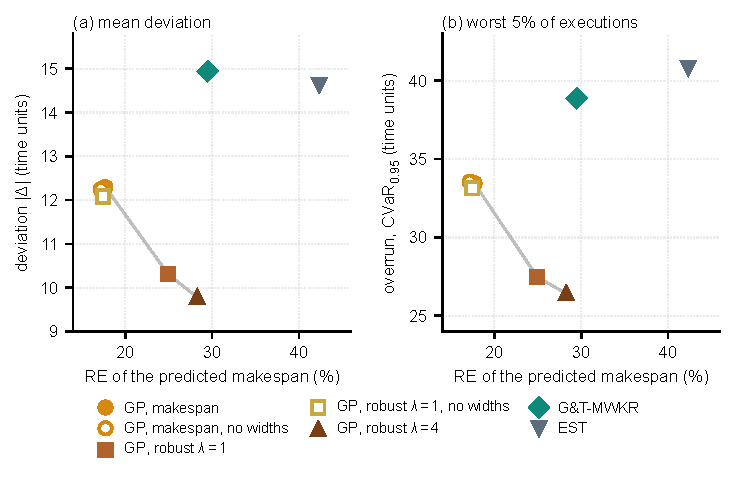
\includegraphics[width=\linewidth]{figures/fig_robustness_plane.pdf}
\caption{Prediction quality against execution reliability over the 70
instances (uniform law): (a) mean absolute deviation of the executed
makespan from the predicted one, (b) mean overrun in the worst $5\%$ of
executions, both in time units. The grey line joins the rules with width
terminals as $\lambda$ grows.}
\label{fig:robplane}
\end{figure}

Table~\ref{tab:robustness} reports $\bar\varepsilon$ for a
representative rule of each arm and for the two strongest baselines.
Under the makespan objective, the featured rule and its ablated
counterpart are statistically indistinguishable ($5.70$ against $5.75$
at the nominal width; paired Wilcoxon over the 70 instances,
$z=-0.17$). Over all 30 rules of each arm, however, the width terminals
reduce the mean $\bar\varepsilon$ from $5.77$ to $5.67$ (Mann--Whitney
$z=-2.40$, $p<0.05$ after Holm's correction; Supplementary
Section~\ref{S-sec:robdetail}). The rule is more robust than G\&T-MWKR
($6.29$, $z=-4.42$, $p<0.001$, $|r|=0.61$) and as robust as EST ($5.66$,
$z=0.42$), whose predicted makespan is far longer. A low deviation does
not require a low makespan, so robustness must be optimized directly,
and the robust fitness achieves this. Over all 30 rules of each arm it
lowers the mean $\bar\varepsilon$ from $5.67$ to $5.50$ (Mann--Whitney
$z=-2.68$, $p<0.05$ after Holm's correction). The narrowest rule of the
$\lambda{=}1$ arm on the validation set reduces it by about a fifth,
from $5.70$ to $4.52$ ($z=-6.40$, $|r|=0.88$ against the makespan rule).
The reduction requires the width terminals: under the same fitness, the
ablated counterpart reaches $5.54$ ($z=-6.25$, $|r|=0.86$). At
$\lambda{=}4$, $\bar\varepsilon$ falls to $4.21$. The ordering holds as the
intervals are widened, and the advantage of the robust rule grows with
the widening: at $+40\%$ its $\bar\varepsilon$ is $6.08$, against $7.57$
for the makespan rule and $8.58$ for G\&T-MWKR.

Figure~\ref{fig:robplane} complements $\bar\varepsilon$ with the
deviation in time units, $|\Delta|$, against the quality of the
prediction. The rule deviates by $12.30$ time units, against $14.64$ for
EST and $14.94$ for G\&T-MWKR. The robust rules move down and to the right along the grey
line: the narrowest rule of the $\lambda{=}1$ arm deviates by $10.31$
time units, $16.2\%$ less than the makespan rule ($z=-5.55$, $p<0.001$,
$|r|=0.76$), and the rule at $\lambda{=}4$ by $9.78$. At matched a-priori
quality the gain is clearest: the $\lambda{=}4$ rule and G\&T-MWKR
predict almost the same makespan, $28.27$ against $29.50$ points of
$\RE$, and the rule deviates $34.5\%$ less, on 69 of the 70 instances
($z=-7.26$, $p<0.001$, $|r|=1.00$). Over the worst $5\%$ of executions
(Figure~\ref{fig:robplane}b) the ordering is the same, and the robust
objective reduces the overrun beyond the prediction in about the same
proportion as the mean deviation, from $33.46$ to $27.46$ time units at
$\lambda{=}1$. In absolute terms, the length of those executions follows
the expected makespan that the robust rules trade for reliability.

Supplementary Section~\ref{S-sec:robdetail} reports the per-instance
distributions, the full comparison over all 30 rules of each arm, and
three other realization laws, under which the ordering and every significant
contrast above hold.

\subsection{Asymmetric intervals}
\label{sec:asym}

All the intervals used so far are symmetric about the crisp duration.
To test whether the contribution of the width terminals depends on that
construction, the four arms of Sections~\ref{sec:ablation}
and~\ref{sec:frontier}, both objectives with and without width
terminals, are re-evolved with fifteen seeds on the right-skewed
versions of TA11--TA14 (Section~\ref{sec:instances}) and evaluated on
the 70 right-skewed instances (Supplementary Section~\ref{S-sec:asym}).
The outcome matches the symmetric case. Under the robust objective the
width terminals narrow the predicted interval from $12.97\%$ to
$12.67\%$ of the expected makespan and reduce the deviation of the
executed makespan, $|\Delta|$, from $13.03$ to $12.75$ time units, both
significant after Holm's correction; under the makespan objective
neither difference is significant. The robustness that the width
terminals provide is therefore not a product of symmetric intervals.

\subsection{Limitations}
\label{sec:limitations}
Four limitations bound the scope of these conclusions. First, the rules
are evolved and applied with the semi-active decoder. Run inside Giffler
and Thompson's active decoder after evolution, the same rules reach
$23.18\%$ $\RE$ instead of $18.99\%$ (Section~\ref{sec:decoder}); rules
evolved directly inside the active decoder have not been tested.

Second, the rules are evolved under the symmetric $\pm15\%$ interval
scheme standard in the IJSP literature. Their robustness ordering holds
under intervals widened by $20\%$ and $40\%$
(Section~\ref{sec:robustness}), and re-evolution on right-skewed
intervals preserves the contribution of the width terminals
(Section~\ref{sec:asym}), but evolution under intervals of a different
magnitude has not been tested.

Third, budgets are measured in seconds of a Python implementation
shared by all methods. In a compiled language such as C++ the curves of
Section~\ref{sec:budget} would converge at lower budgets; the comparison
itself changes only if the language alters the cost of a schedule
built by the rule relative to one decoded by the genetic algorithm. The
rankings of the other sections do not depend on time.

Finally, no learned policy is among the baselines. The only
reinforcement-learning method published for the
IJSP~\citep{Han2026RAPO} leaves part of the sequencing to be resolved
during execution, so it does not belong to the single-pass class
compared here, and it reports results on a different selection of
classical instances.

\section{Conclusions and Future Work}
\label{sec:conclusions}

We presented a GP hyper-heuristic for job shop scheduling with interval
durations, which evolves priority rules over a terminal set exposing
both the worst-case values and the widths of the uncertain quantities.
The evolved rules are compact enough to be read and simplified by hand.
In a single constructive pass they average $18.99\%$ $\RE$ over 30 evolutions,
and the featured rule attains $17.71\%$, against $29.5\%$ for the strongest
baseline, G\&T-MWKR; the featured rule outperforms every deterministic
constructive baseline on all 70 interval Taillard instances. Evolved on four $20{\times}15$
instances, the rules transfer without retraining to every size class and
to the classical instances, and perform best on the unseen
$50{\times}15$ class.

The questions of Section~\ref{sec:intro} receive the following answers.
First, the evolution selects the classical scheduling attributes most
often, slack, work remaining, earliest start and processing time, and
keeps the width terminals in most rules. Second, under the default
expected-makespan objective the magnitude of the uncertainty is not
needed to dispatch well: rules evolved without the width terminals, or
on the crisp midpoint instances, perform as well as the interval-aware
ones. Third, an objective that rewards a narrow makespan interval leads to
more predictable executions. With $\lambda = 1$ the predicted intervals
become narrower and the executions deviate less from them: over the 30
rules of each arm the mean relative deviation $\bar\varepsilon$ falls
from $5.67$ to $5.50$, and the narrowest rule on the validation set
reduces it by about a fifth, a reduction that extends to the worst $5\%$
of executions and grows as the intervals are widened. The expected makespan rises in exchange, by an
amount that the weight $\lambda$ controls. The reduction requires the
width terminals, on symmetric and on asymmetric intervals alike, so it
is under this objective that the magnitude of the uncertainty becomes
useful information.

Fourth, the place of evolved rules among per-instance methods depends on
the budget. Compared with our implementation of the genetic algorithm
published for the IJSP, which shares decoder, evaluator and language
with the rule, GP-best-of-$N$ attains the lowest $\RE$ up to a budget
that grows with instance size, from about $10$~s per instance on the
classical instances to about $300$~s on $50{\times}15$, and a single
pass delivers in milliseconds a quality that the genetic algorithm needs
between $2$ and $46$~s per instance to reach. As a seed, the rule speeds
up the early search of the genetic algorithm. At larger budgets the
genetic algorithm attains a lower $\RE$, and the published ABC variants,
which combine population search with local search, obtain the best
results. Evolved rules are therefore a high-quality, interpretable
method that decides in milliseconds and complements per-instance search,
suited to settings in which schedules must be built or rebuilt quickly.

Future work follows four lines. First, refining the numeric weights of
evolved rules, which the sensitivity analysis of
Section~\ref{sec:anatomy} shows the evolution does not always leave at
their best values; since only the relative weights of the terms affect
the dispatching decisions, a local search over them is the natural
complement.
Second, evolving rules inside Giffler and Thompson's active decoder and
under intervals of other magnitudes, the two settings that
Section~\ref{sec:limitations} leaves open. Third, seeding the published
ABC variants with the rule and with the diverse pools of sequences that
GP-best-of-$N$ produces, and richer symbolic models such as ensembles of
complementary rules~\citep{GilGala2021Ensembles}. Fourth, a controlled
comparison with learned neural constructive policies under matched
training and inference budgets, the evaluation that the recent
literature~\citep{Xu2025} identifies as missing.

\section*{CRediT authorship contribution statement}
\textbf{Hern\'an D\'iaz}: Conceptualization, Methodology, Software,
Validation, Formal analysis, Investigation, Resources, Data curation,
Writing -- original draft, Writing -- review \& editing, Visualization.

\section*{Acknowledgements}
This work was supported by the Spanish Ministry of Science, Innovation
and Universities (MCIN/AEI/10.13039/501100011033) under grant
PID2022-141746OB-I00.

\section*{Declaration of competing interest}
The author declares that there are no known competing financial
interests or personal relationships that could have appeared to
influence the work reported in this paper.

\section*{Data availability}
The GP hyper-heuristic is implemented from scratch in pure Python/NumPy,
with no evolutionary-computation dependencies; evolved rules are stored
as plain JSON expression trees and evaluated as drop-in dispatching
strategies. All benchmark
instances, the 430 evolved rules of every experimental arm, the primary
result files behind each table and figure, and a self-contained
implementation that re-derives the deposited results from scratch are
openly available in a Zenodo repository~\citep{DiazDataset2026}
(\href{https://doi.org/10.5281/zenodo.21716972}{doi:10.5281/zenodo.21716972}).
Version 2.0 of the repository
(\href{https://doi.org/10.5281/zenodo.23156759}{doi:10.5281/zenodo.23156759})
holds the material of this article, including its supplementary
material.

\section*{Declaration of generative AI and AI-assisted technologies in
the manuscript preparation process}
During the preparation of this work the author used Claude (Anthropic)
in order to assist with the drafting and editing of the manuscript.
After using this tool, the author reviewed and edited the content as
needed and takes full responsibility for the content of the published
article.

\bibliographystyle{elsarticle-harv}
\bibliography{refs}

\end{document}
